\section*{АЛУ К155ИП3}
\addcontentsline{toc}{section}{АЛУ К155ИП3}
\subsection*{Построение демонстрационной модели К155ИП3}
\addcontentsline{toc}{subsection}{Построение демонстрационной модели К155ИП3}

Ниже, на рисунке \ref{image:5} представленна демонстрационная модель АЛУ К155ИП3.\par

\begin{figure}[h]
    \centering
    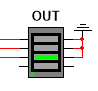
\includegraphics[scale=0.8]{image-5.png}
    \caption{АЛУ К155ИП3}
    \label{image:5}
\end{figure}

Данная модель имеет несколько групп входных и выходных сигналов:

\begin{itemize}
    \item A1-A4 \textbf{---} информационные входы первого операнда
    \item B1-B4 \textbf{---} информационные входы второго операнда
    \item F0-F3 \textbf{---} исполняемая операция
    \item $\overline{Z}$ \textbf{---} вход переноса
    \item M \textbf{---} режим работы АЛУ. $M=0$ - арифметический, $M=1$ - логический
    \item S1-S4 \textbf{---} результат операции
    \item $\overline{P}$ \textbf{---} выход переноса
\end{itemize}

\newpage
\subsection*{Тестирование арифметических операций К155ИП3}
\addcontentsline{toc}{subsection}{Тестирование арифметических операций К155ИП3}

Протестируем работу АЛУ на примере следующих арифметических операций:

\begin{table}[h!]
    \begin{center}
        \begin{tabular}{ 
            |>\centering m{1cm}
            |>\centering m{1cm}
            |>\centering m{1cm} 
            |>\centering m{1cm} 
            |>\centering m{1cm} 
            |>\centering m{1cm} 
            | m{2cm}
            | 
        }
            \hline
              &   &   &   &   &   &  \arraybackslash \\[-0.4cm]
            № & $\overline{Z}$ & F0 & F1 & F2 & F3 & \centering Операция \arraybackslash \\ \hline
            1 & 0 & 0 & 1 & 1 & 0 & \centering $A-B$ \arraybackslash \\ \hline
            2 & 0 & 1 & 0 & 0 & 1 & \centering $A+B+1$ \arraybackslash \\ \hline
            3 & 1 & 0 & 0 & 1 & 1 & \centering $A+A$ \arraybackslash \\ \hline
        \end{tabular}
        \caption{Таблица арифметических операций для тестирования АЛУ}
        \label{table:3}
    \end{center}    
\end{table}

\textbf{Рассмотрим операцию №1.} Выставим режим работы АЛУ в арифметический ($M=0$), 
в группе входов F укажем режим работы (0110). Подадим на группу входных сигналов A значение 15 (1111), на группу B 6(0110). 
По результатам операции $A-B$ ожидаем получить 9(1001). \par
 
\begin{figure}[h]
    \centering
    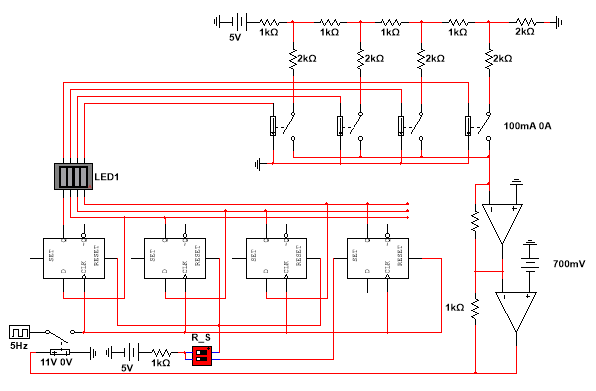
\includegraphics[scale=0.8]{image-6.png}
    \caption{Арифметическая операция №1}
    \label{image:6}
\end{figure}

На панели индикации видим управляющи сигнал 1001(9), что соответвует ожидаемому результату. \par

\newpage
\textbf{Рассмотрим операцию №2.} Переключатели группы F выставим в режим работы второй операции (1001). 
Значения для тестирования возьмем $A=5,B=5$. Ожидаемый результат $A+B+1=5+5+1=11$. \par

\begin{figure}[h]
    \centering
    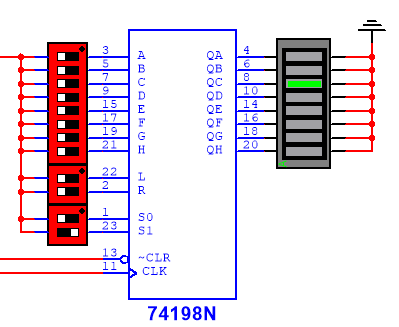
\includegraphics[scale=0.8]{image-7.png}
    \caption{Арифметическая операция №2}
    \label{image:7}
\end{figure}

На панели индикации видим управляющи сигнал 1011(11), что соответвует ожидаемому результату. \par

\textbf{Рассмотрим операцию №3.} Переключатели группы F выставим в режим работы третьей операции (0011). 
Значения для тестирования возьмем $A=6$. Ожидаемый результат $A+A=6+6=12$. \par

\begin{figure}[h]
    \centering
    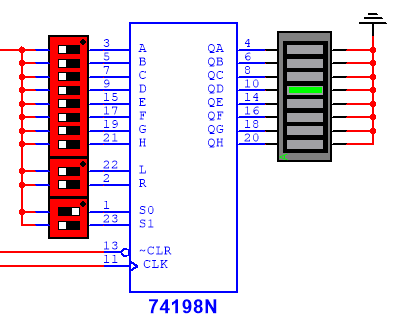
\includegraphics[scale=0.8]{image-8.png}
    \caption{Арифметическая операция №3}
    \label{image:8}
\end{figure}

На панели индикации видим управляющи сигнал 1100(12), что соответвует ожидаемому результату. \par

\newpage
\subsection*{Тестирование логических операций К155ИП3}
\addcontentsline{toc}{subsection}{Тестирование логических операций К155ИП3}

Протестируем работу АЛУ на примере следующих логических операций:

\begin{table}[h!]
    \begin{center}
        \begin{tabular}{ 
            |>\centering m{1cm}
            |>\centering m{1cm} 
            |>\centering m{1cm} 
            |>\centering m{1cm} 
            |>\centering m{1cm} 
            | m{2cm}
            | 
        }
            \hline
            &   &   &   &   &  \arraybackslash \\[-0.4cm]
            № & F0 & F1 & F2 & F3 & \centering Операция \arraybackslash \\ \hline
            &   &   &   &   &  \arraybackslash \\[-0.4cm]
            1 & 0 & 1 & 1 & 0 & \centering $A \oplus B$ \arraybackslash \\ \hline
            &   &   &   &   &  \arraybackslash \\[-0.4cm]
            2 & 1 & 1 & 0 & 1 & \centering $AB$ \arraybackslash \\ \hline
            &   &   &   &   &  \arraybackslash \\[-0.4cm]
            3 & 0 & 1 & 1 & 1 & \centering $A \vee B$ \arraybackslash \\ \hline
        \end{tabular}
        \caption{Таблица логических операций для тестирования АЛУ}
        \label{table:4}
    \end{center}    
\end{table}

\textbf{Рассмотрим операцию №1.} Переключим режим работы АЛУ в логический ($M=1$).
Для тестирвания возьмем значения $A=0011,B=0101$. В результате ожидаем:

$$
    \begin{array}{r}
        \oplus
        \begin{array}{r}
            0011 \\
            0101
        \end{array} \\
        \hline
        \begin{array}{r}
            0110
        \end{array}
    \end{array}
$$

Выставив функцию №1 на блоке F проверим результат.
\begin{figure}[h]
    \centering
    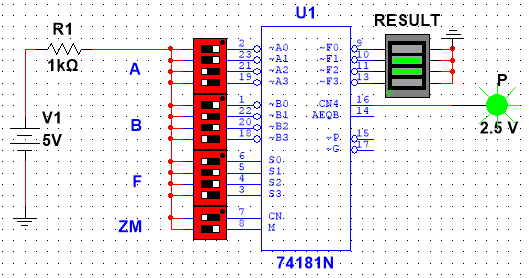
\includegraphics[scale=0.8]{image-9.png}
    \caption{Логическая операция №1}
    \label{image:9}
\end{figure}

На панели индикации видим управляющи сигнал 0110, что соответвует ожидаемому результату. \par

\newpage
\textbf{Рассмотрим операцию №2.} Выставим блок F для операции №2 (1101).
Возьмем значения $A=0110,B=1101$. Ожидаемый результат:
$$
    \begin{array}{r}
        \wedge
        \begin{array}{r}
            0110 \\
            1101
        \end{array} \\
        \hline
        \begin{array}{r}
            0100
        \end{array}
    \end{array}
$$

\begin{figure}[h]
    \centering
    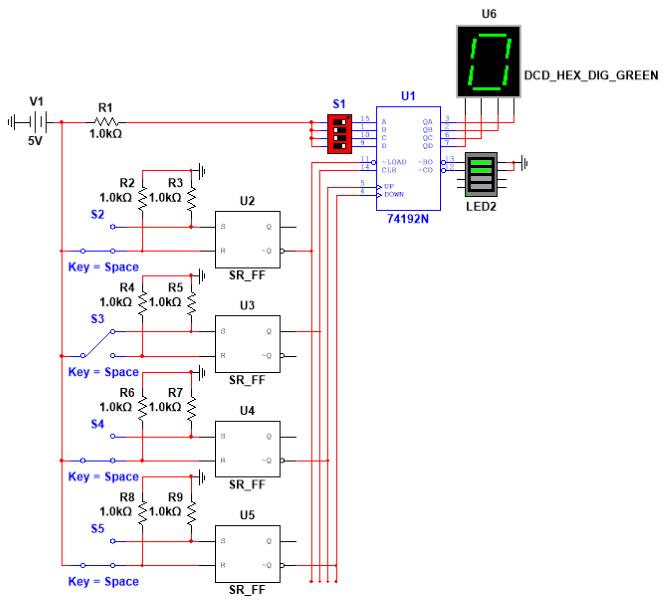
\includegraphics[scale=0.8]{image-10.png}
    \caption{Логическая операция №2}
    \label{image:10}
\end{figure}

На панели индикации видим управляющи сигнал 0100, что соответвует ожидаемому результату. \par

\textbf{Рассмотрим операцию №3.} Выставим блок F для операции №3 (0111).
Возьмем значения $A=1010,B=0111$. Ожидаемый результат:
$$
    \begin{array}{r}
        \vee
        \begin{array}{r}
            1010 \\
            0111
        \end{array} \\
        \hline
        \begin{array}{r}
            1111
        \end{array}
    \end{array}
$$

\begin{figure}[h]
    \centering
    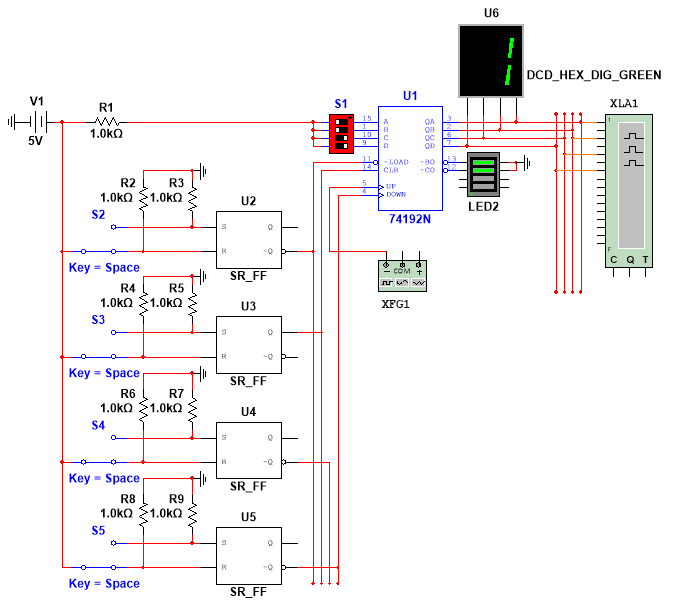
\includegraphics[scale=0.8]{image-11.png}
    \caption{Логическая операция №3}
    \label{image:11}
\end{figure}

На панели индикации видим управляющи сигнал 1111, что соответвует ожидаемому результату. \par

\newpage